\documentclass[12pt,a4 paper]{report}  % To indicate fontsize, page type and document type
\renewcommand{\baselinestretch}{1.5} % To make the linespacing in the document 1.5cm
%\renewcommand{\bibname}{}  % To make title "BIBLIOGRAPHY" to "REFERENCES"
%\usepackage{amsmath,graphicx,color,geometry,fancyhdr,subfigure}
\usepackage{amsmath,epsfig,cite,graphicx,ltablex,tabularx,setspace,url,
floatflt,caption,float,comment,fancyhdr,geometry,subfigure,amssymb,color,indentfirst,booktabs,array,xspace}
%\usepackage[caption=false,font=footnotesize]{subfig}
\DeclareMathOperator*{\esup}{argmax}
%\usepackage{amsmath,graphicx,color,geometry,subfigure}
%  'amsmath'   --   for [equation*]
%  'graphicx'    --   To include figures
%  'color'          --   To include texts with color and also with different fonts
%  'geometry'   --   To change page properties
%  'fancyhdr'    --   To make the pages look good by including special effects
%  'subfigure'   --   To include two figures in a single figure
% INCLUDE subfigure after fancyhdr since now it is not working because packages are not updated fully.

\geometry{left=1.25in,right=1in}
\geometry{top=1.1in,bottom=1in}       % page geometry

\setcounter{secnumdepth}{3}%
% to get subsubsections numbered
\setcounter{tocdepth}{3}%
% to get subsubsections in the table of contents

% Project Details
\newcommand{\projectName}{DaxOS\xspace}

\newcommand{\firstAuthor}{Nihal Narayan\xspace}
\newcommand{\firstAuthorRegNo}{MBT17CS081\xspace}

\newcommand{\secondAuthor}{Antony S. Chirayil\xspace}
\newcommand{\secondAuthorRegNo}{MBT17CS023\xspace}

\newcommand{\thirdAuthor}{Mathew Koshy\xspace}
\newcommand{\thirdAuthorRegNo}{MBT17CS068\xspace}

\newcommand{\fourthAuthor}{R Midhun Suresh\xspace}
\newcommand{\fourthAuthorRegNo}{MBT17CS095\xspace}

\begin{document}  % actual document beginning
\renewcommand\bibname{REFERENCES}

%-----COVER PAGE-----%
\begin{titlepage}
\begin{center}
{\Large\sf \textbf{\textcolor[rgb]{0,0,0}{{DaxOS}}}}\\[5ex]
\vspace{0.3 cm}
A PROJECT REPORT\\
submitted by

{\small \textcolor[rgb]{0,0,0}{\emph{By}} \\[1ex]

{\sf \sf {\textcolor[rgb]{0,0,0}{Nihal Narayan (MBT17CSXX) \\ Antony S. Chirayil (MBT17CSXX) \\ Mathew Koshy (MBT17CSXX) 
			\\ R Midhun Suresh (MBT17CS095)}}} \\% Enter the name of author
\vspace{0.5 cm}
to
\\
\vspace{0.5 cm}
\textbf{the APJ Abdul Kalam Technological University \\
	in partial fulfillment of the requirements for the award of the Degree }\\
\vspace{0.8 cm}
of
\\
 
%\vspace{0.8 cm}
%\\
%\textbf{FACULTY OF COMPUTER SCIENCE AND ENGINEERING}

%\textit{\textcolor[rgb]{0,0,0}{{In partial fulfillment of the requirements \\ for the award of the degree\\ of} \\}}
\textbf{BACHELOR OF TECHNOLOGY}}
\\
IN 
\\
\textit{COMPUTER SCIENCE AND ENGINEERING}
\\
    \textbf{ May, 2019}
% DEPT: Enter the name of Department,  SPECIALIZATION: Enter the specialization, 
\vspace{0.2 cm} \\[2ex]

 \begin{figure}[ht]
 \begin{center}
\resizebox{2in}{!}{
\includegraphics{mbcetlogo-eps-converted-to}}
 \end{center}
 \end{figure}

{\sf \textbf{\textcolor[rgb]{0,0,0}{DEPARTMENT OF COMPUTER SCIENCE AND ENGINEEERING}}}\\[0.5ex]
{\sf {\textcolor[rgb]{0,0,0}{MAR BASELIOS COLLEGE OF ENGINEERING \& TECHNOLOGY}}}\\[0.4ex]
Bethany Hills, Nalanchira\\
{\sf \textcolor[rgb]{0,0,0}{Thiruvananthapuram 15}}\\[0.5ex]

\end{center}
\end{titlepage}


%-----COVER PAGE-----%

%-----CERTIFICATE-----%
\thispagestyle{empty}

\setlength{\headsep}{0.4in}
\begin{center}

{\sf \textbf{\textcolor[rgb]{0,0,0}{DEPARTMENT OF COMPUTER SCIENCE AND ENGINEERING}}}\\[0.5ex]
{\sf{\textcolor [rgb]{0,0,0} MAR BASELIOS COLLEGE OF ENGINEERING \& TECHNOLOGY}}\\[0.4ex]
Nalanchira, Thiruvananthapuram.



\end{center}


\vspace{0.15cm}
 \begin{figure}[!h]
 \begin{center}
\resizebox{2in}{!}{
\includegraphics{mbcetlogo-eps-converted-to}}
 \end{center}
 \end{figure}
\vspace{0.02cm}

\begin{center}
\textcolor[rgb]{0,0,0}{\textbf{\underline{CERTIFICATE}}} \\[1ex]
\end{center}
\par

\emph{
\textit{{This is to certify that the report entitled \textbf{\projectName}  submitted by \textbf{\firstAuthor(\firstAuthorRegNo)},
		\textbf{\secondAuthor(\secondAuthorRegNo)},
		\textbf{\thirdAuthor \\ (\thirdAuthorRegNo)},
		\textbf{\fourthAuthor(\fourthAuthorRegNo)}
		 to the APJ Abdul Kalam Technological University in partial fulfillment of the
		requirements for the award of the Degree of {Bachelor of Technology} in {Computer Science and Engineering and Technology} is a bonafide record of the project work carried out by him/her under my/our guidance and supervision.This report in any form has not been submitted to any other University or Institute for any purpose}}} 



\vspace{3.0 cm}



\begin{tabular*}{\textwidth}{c @{\extracolsep{\fill}} ccc}
	\textbf{Ms. Gayathri K. S.} & 	\textbf{Mr. V. S. Shibu} & 	\textbf{Dr. Tessy Mathew} \\ 
	Project Coordinator & Guide & Head of the Department 
\end{tabular*}


\vspace{2.0 cm}

\begin{flushleft}
\textit{\textbf{Place: Thiruvananthapuram}} \\
\textit{\textbf{Date: 12/01/2021}}	
\end{flushleft}






%-----CERTIFICATE-----%

\pagenumbering{roman}   % to get page numbers for initial pages in terms of roman numbers
%-----ACKNOWLEDGEMENTS-----%
% Thesis - Abstract
\chapter*{\centering Acknowledgement}

\begin{flushleft}
	 We would like to take this opportunity to extend our sincere gratitude to \textbf{Mr. Shibu VS} for guiding us through the process of this project.
	 We would also like to thank the seminar coordinator, \textbf{Mrs. Gayathri KS}, for providing us with this opportunity which has allowed us to explore a domain which would otherwise be beyond the confines of our academic course.
\end{flushleft}

















%-----ACKNOWLEDGEMENTS-----%

%-----ABSTRACT-----%
% Thesis - Abstract
\section*{\centering ABSTRACT}

\indent {
Every computer science enthusiast is proficient in their operating system of choice. They may
even know its underlying working from an old operating system course they took in college.
However, it is usually the case that their knowledge and understanding is limited to theory and
writing low-level system code is often considered an insurmountable challenge.
This project hopes to change this attitude by developing a minimal yet functional 32-bit
operating system that can be used in conjunction with theoretical teaching to promote and
introduce systems programming. A minimal kernel guarantees easier to read source code (as
opposed to the 27 million SLOC Linux kernel) and provides a gentler introduction to kernel
development.
The kernel will include a full keyboard and mouse driver and will have support for VGA
text-mode and graphics. It will also contain a limited libc implementation with a streamlined
build process.
Additionally, this project will serve as an illustration for good development practices (code
reuse, clean architecture, unit testing).
The 32-bit kernel will be written in C with a little of assembly for the
truly low-level aspects. 
}

%-----ABSTRACT-----%

\tableofcontents

\clearpage
\addcontentsline{toc}{chapter}{List of Figures}
\listoffigures

\clearpage
\addcontentsline{toc}{chapter}{List of Tables}
\listoftables
\clearpage
\addcontentsline{toc}{chapter}{Nomenclature}
\section*{\centering Nomenclature}
\vspace{1.5 cm}

\begin{flushleft}
	

$GDT$   \hspace{1.0 cm} Global Descriptor Table\\
$IDT$   \hspace{1.0 cm} Interrupt Descriptor Table\\
$ISR$   \hspace{1.0 cm} Interrupt Service Routine\\
$VGA$   \hspace{1.0 cm} Video Graphics Array\\
$APM$   \hspace{1.0 cm} Advanced Power Management\\



\end{flushleft}
\newpage
\pagenumbering{arabic}
\pagestyle{fancy}                       % Sets fancy header and footer
\fancyfoot{}                            % Delete current footer settings
\fancyhead{}                            % Delete current footer settings
\rhead{project title}		% Write your thesis topic here
\lfoot{Dept: of {Computer Science and Engineering}}
\rfoot{ \thepage}
\renewcommand{\headrulewidth}{0.4pt}
\renewcommand{\footrulewidth}{0.4pt}
\renewcommand{\pagenumbering}{} 

\chapter{Introduction}\label{chapter:Introduction}


\indent{
The Kernel is the fundamental interconnect between hardware and software of a computer system. 
Writing a kernel (kernel programming) is considered to be a difficult endeavor because development has to start from a bare metal state. 
DAX OS is a minimal 32-bit hobbyist operating system that can be used to provide a gentle introduction to students who wish to explore the domain of systems programming.

The project is open source and licensed under GNU General Public License v3.0 to ensure unrestricted access and complete transparency. 
DAX OS comes with a terminal driver, keyboard and mouse driver and basic memory management.
The project also uses appropriate development practises such as unit-testing and version control.}

Some key facts about this project are:
\begin{itemize}
	\item Source code is hosted at \url{https://github.com/DaxKernel/OS}.
	\item About 2500 lines of code only
	\item 32-bit
	\item Low resource consumption
\end{itemize}

\newpage
\section{Objectives}\label{section:Objectives}
We propose to build a 32-bit kernel that has the following functionality:
\begin{enumerate}
	
	\item \textbf{Keyboard Driver} \\
	Dax-OS includes a fully functional PS/2 keyboard driver. The PS/2 keyboard driver will convert scan-codes generated when the user presses a key on the keyboard to an integer character code. It must be noted that all keyboards practically used in modern day utilize the USB standard. We stick with the PS/2 protocol because the USB protocol is massive and difficult to implement. However there are practically no disadvantages from such a decision because most motherboards will emulate USB keyboards as PS/2 keyboards.
	
	\item \textbf{Terminal Display Driver} \\
	DaxOS is a terminal based operating system i.e it does not support windowing.
	The display support will be implemented using VGA text-mode and real-mode.
	It will later be re-implemented in Graphics.
	
	\item \textbf{Interrupts}  \\
	DaxOS makes heavy use of interrupts for device drivers. It also uses interrupts for handling CPU exceptions. 

	\item \textbf{Memory Management} \\
	DaxOS uses a flat memory model.
	Since it is an 32-bit operating system, it will support at most 4GB of addressable memory. 
	A custom memory allocator has also be implemented.

	\item \textbf{Graphics Support} \\
	DaxOS will provide graphics capability using VESA mode. The supported resolution is 1280x720. 

	\item \textbf{Font Rendering} \\
	With graphics support, the vga text-mode based terminal driver is depreciated in favor of the higher resolution VESA mode.
	Font rendering needed for this scenario is also available.

	\item \textbf{Image Rendering} \\
	DaxOs will natively support rendering images in TGA format.
\end{enumerate}

\section{Limitations} \label{section:Limitations}
Some functionality DaxOS does not implement are:
\begin{itemize}
	\item Process Management
	\item GUI
	\item Paging
\end{itemize}

\section{Technology Stack} \label{section:Technology Stack}
The bulk of the operating system is written in the C programming language.
Certain functionality such as writing data to ports and loading tables (IDT, GDT) are implemented using either GCC inline assembly or using normal x86 assembly.

The project uses the GCC cross-compiler \& binutils to target the generic i686 platform; which is a generic 32-bit Intel P6 architecture.
The GNU Assembler and Linker are also used. The assembly syntax style used is AT\&T.

The entire compilation process is driven using GNU Make which uses Makefiles to build the project.
The compilation is initiated using BASH shell scripts.
The kernel is tested using the qemu-i386 emulator and is developed on a stable Xubuntu distribution. 

DAX OS uses git as its version control system of choice.
The git repository is uploaded on Github and every new feature is developed on its own separate branch.
Team communication and coordination are actualized using discord with Github integration enabled.




\chapter{Literature Review}\label{chapter:Literature Review}
\indent Write the literature review here.

\indent Citations should be included as \cite{Chen}, or \cite{Kondoz,atal} if there are more than one references to cite.

\indent 



\chapter{Chapter heading}
\indent Write the body of the thesis. Include as many chapters as needed.


\section{Sections in chapter}

Logically divide the content of the chapter into sections and subsections. 


\subsection{An example subsection}

Within a subsection, content division may again be included as shown below.

\subsubsection{Examples of equations}

\indent  A few examples of various types of equations are shown in Eq.~\ref{eq:A(z)}, to Eq.~\ref{eq:vs1}.

\begin{equation}
  	A(\emph{z})= \frac{1-B(\emph{z})}{1-B(\frac{z}{\gamma})}
  	\label{eq:A(z)}
\end{equation}

\begin{equation}
	A(\frac{z}{\gamma})=\sum\limits_{i=1}^M \gamma^{i} x_{i}z^{-i}, 0 < \gamma < 1
  	\label{eq:A(z/gamma)}
\end{equation}

\begin{equation}
  	a_{n}^{'}=
	\begin{cases}

	a_{n}b_{n},& 0\le{n}\le{N-1}\\
   	 0,              & \text{otherwise}
	\end{cases}
  \label{eq:andash}
  \end{equation}


\begin{equation}
  a_{n}= \alpha - \beta \cos \frac{2 \pi n}{N-1}
  \label{eq:an}
  \end{equation}
where \(\alpha = 0.54\) and \(\beta = 1-\alpha = 0.46\).


\begin{equation}
\frac{\delta C}{\delta a_{k}} = 2E[(s[n] + \sum\limits_{k=1}^M (a_{k}s_{n-k}))b_{n-i}] = 0
  \label{eq:dC}
  \end{equation}

\begin{equation}
A=\lVert \mathbf{x}(n) - \eta_{k}b_{i}\mathbf{C}y_j \rVert 
  \label{eq:Alvert}
  \end{equation}

\begin{equation}
  a_{1}= b[T^{(1)}]
  \label{eq:vs1}
  \end{equation}

\subsubsection{Examples of figures}

\indent Figures may be included as in Fig.~\ref{fig:CELPdecth}. To increase or decrease the size of the figures, adjust the `scale' parameter in the code. 
\begin{figure}[h]
      \begin{center}
                 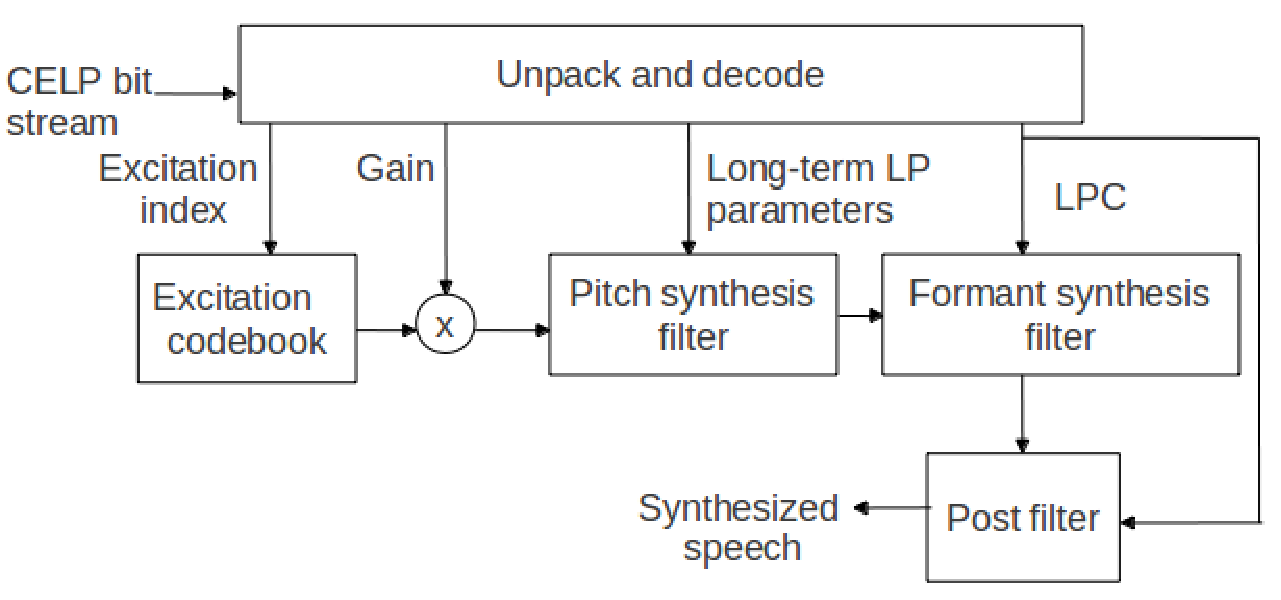
\includegraphics[scale=.55]{CELPdecth-eps-converted-to.pdf}
                 \caption[An Example Figure]{An Example Figure}
		% \label{fig:CELPdecth}
      \end{center}
\end{figure}

\indent If the size of the figures needs to be made uniform, use the parameters `width' and `height' as shown in Fig.~\ref{fig:int}.

\begin{figure*}[h]
\centerline{\subfigure[Original Sound File]{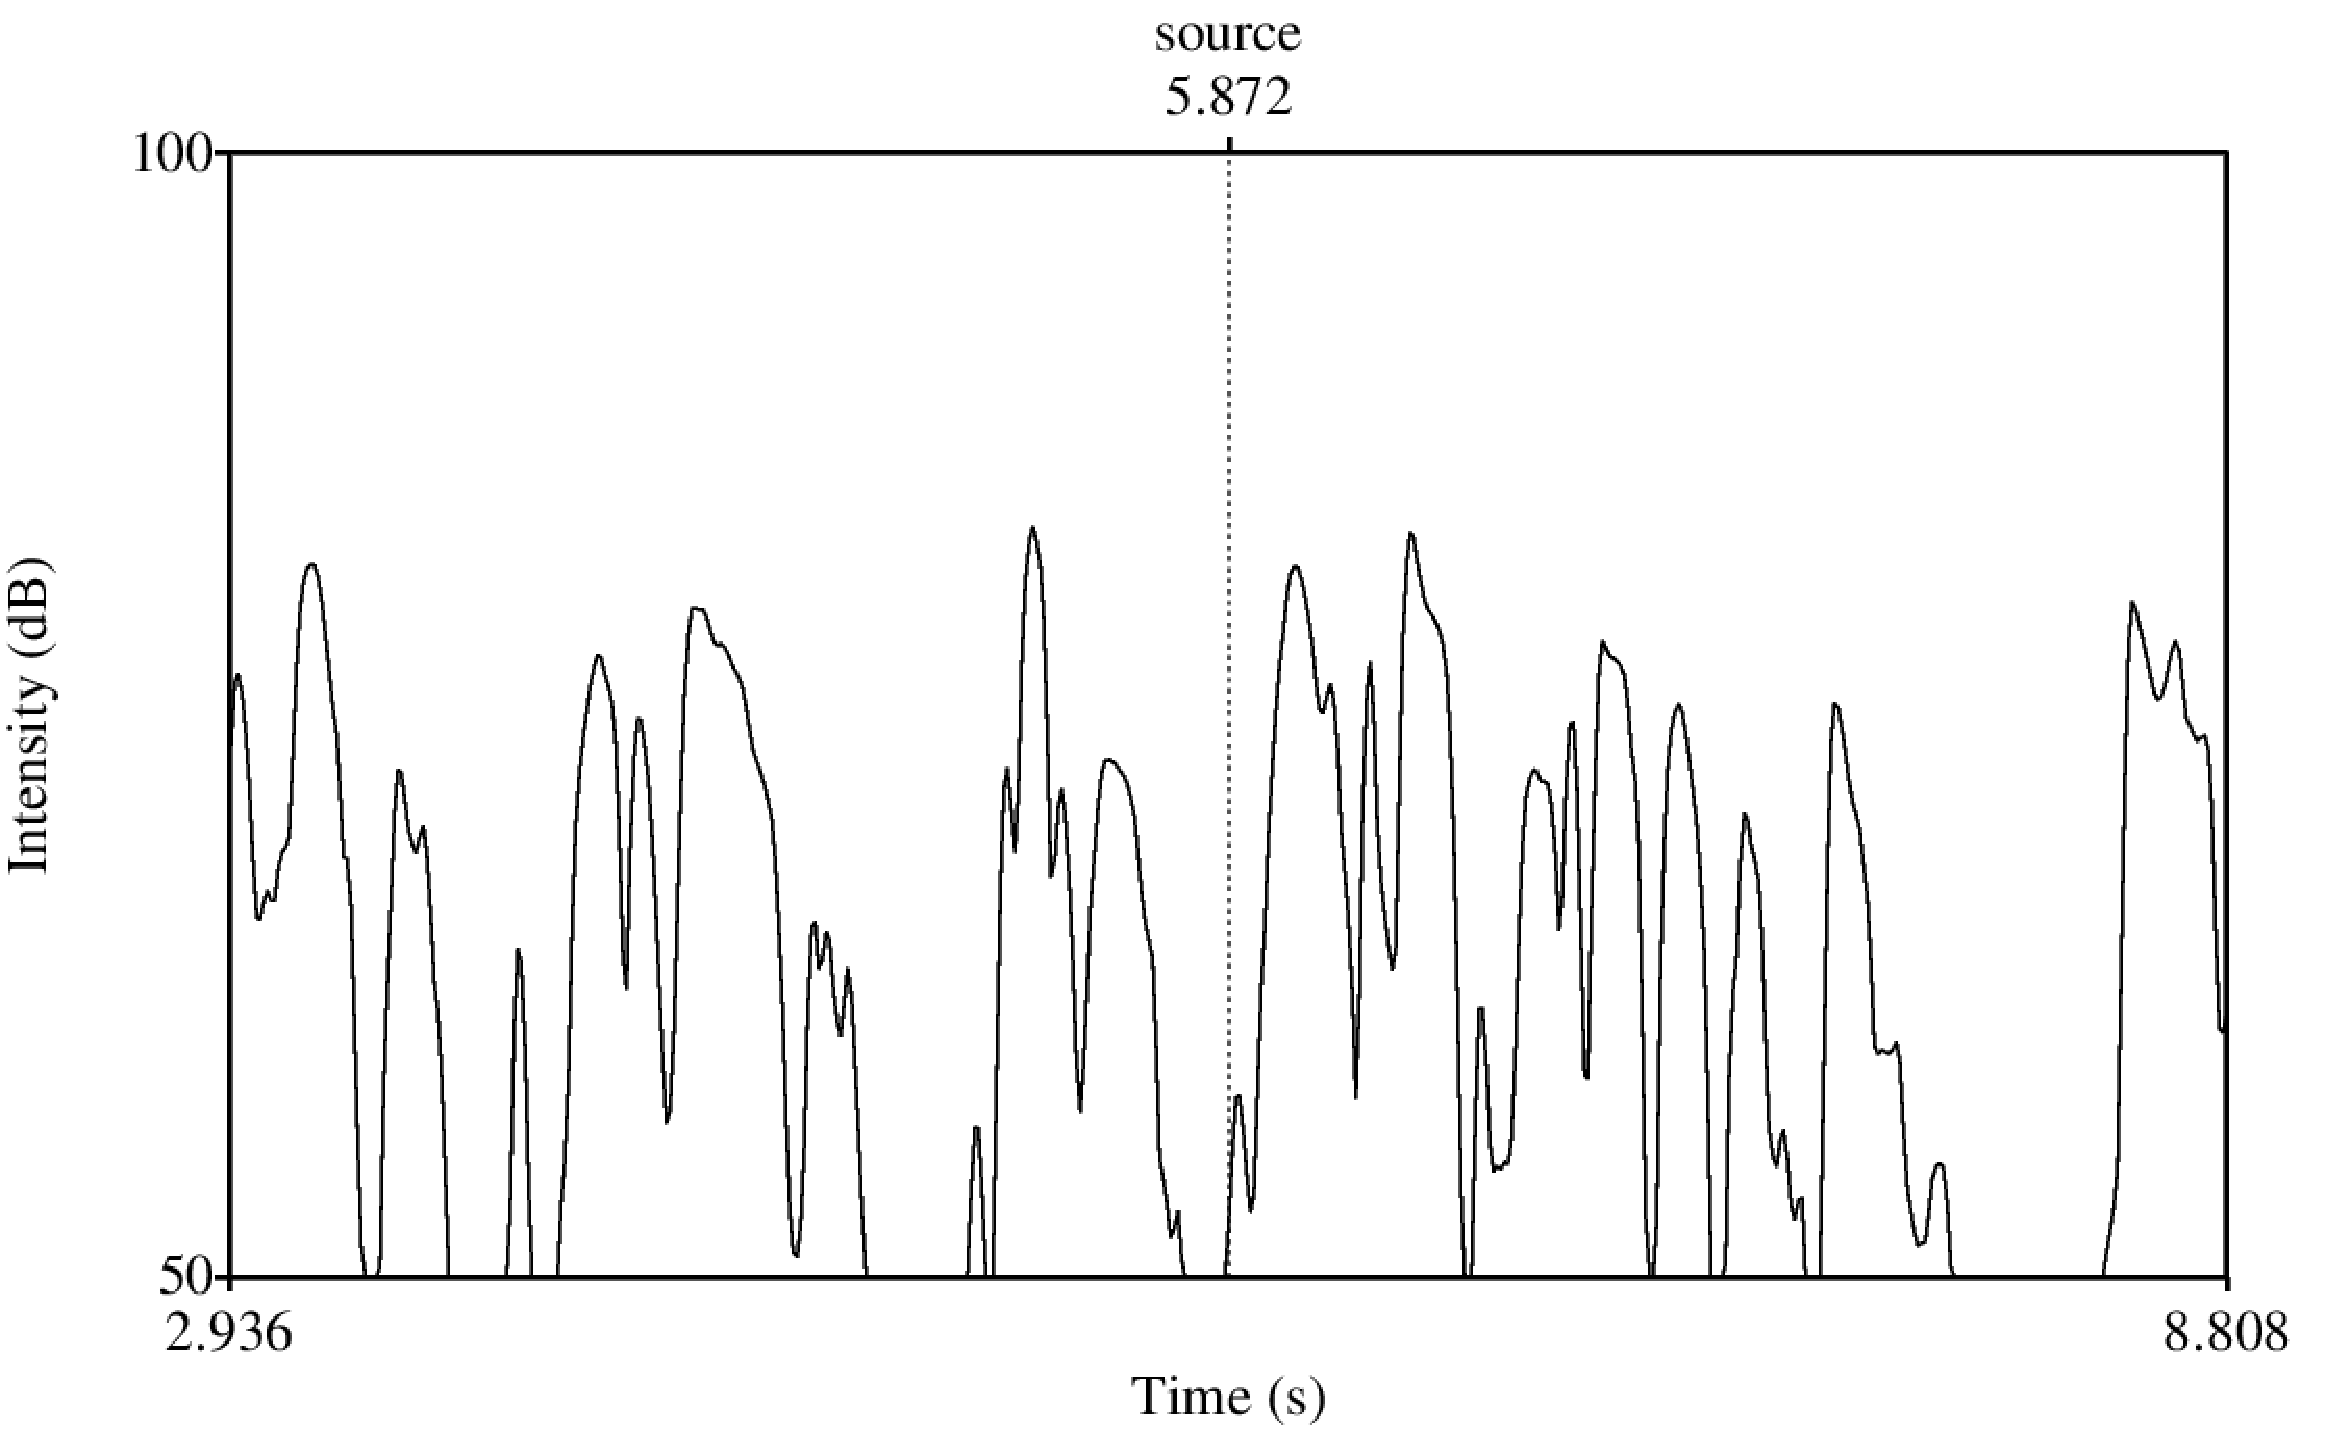
\includegraphics[width=4.5cm, height=3cm]{intorig-eps-converted-to.pdf}%
%\label{fig:intorig}
}
\hfil
\subfigure[Decoder 1 output file]{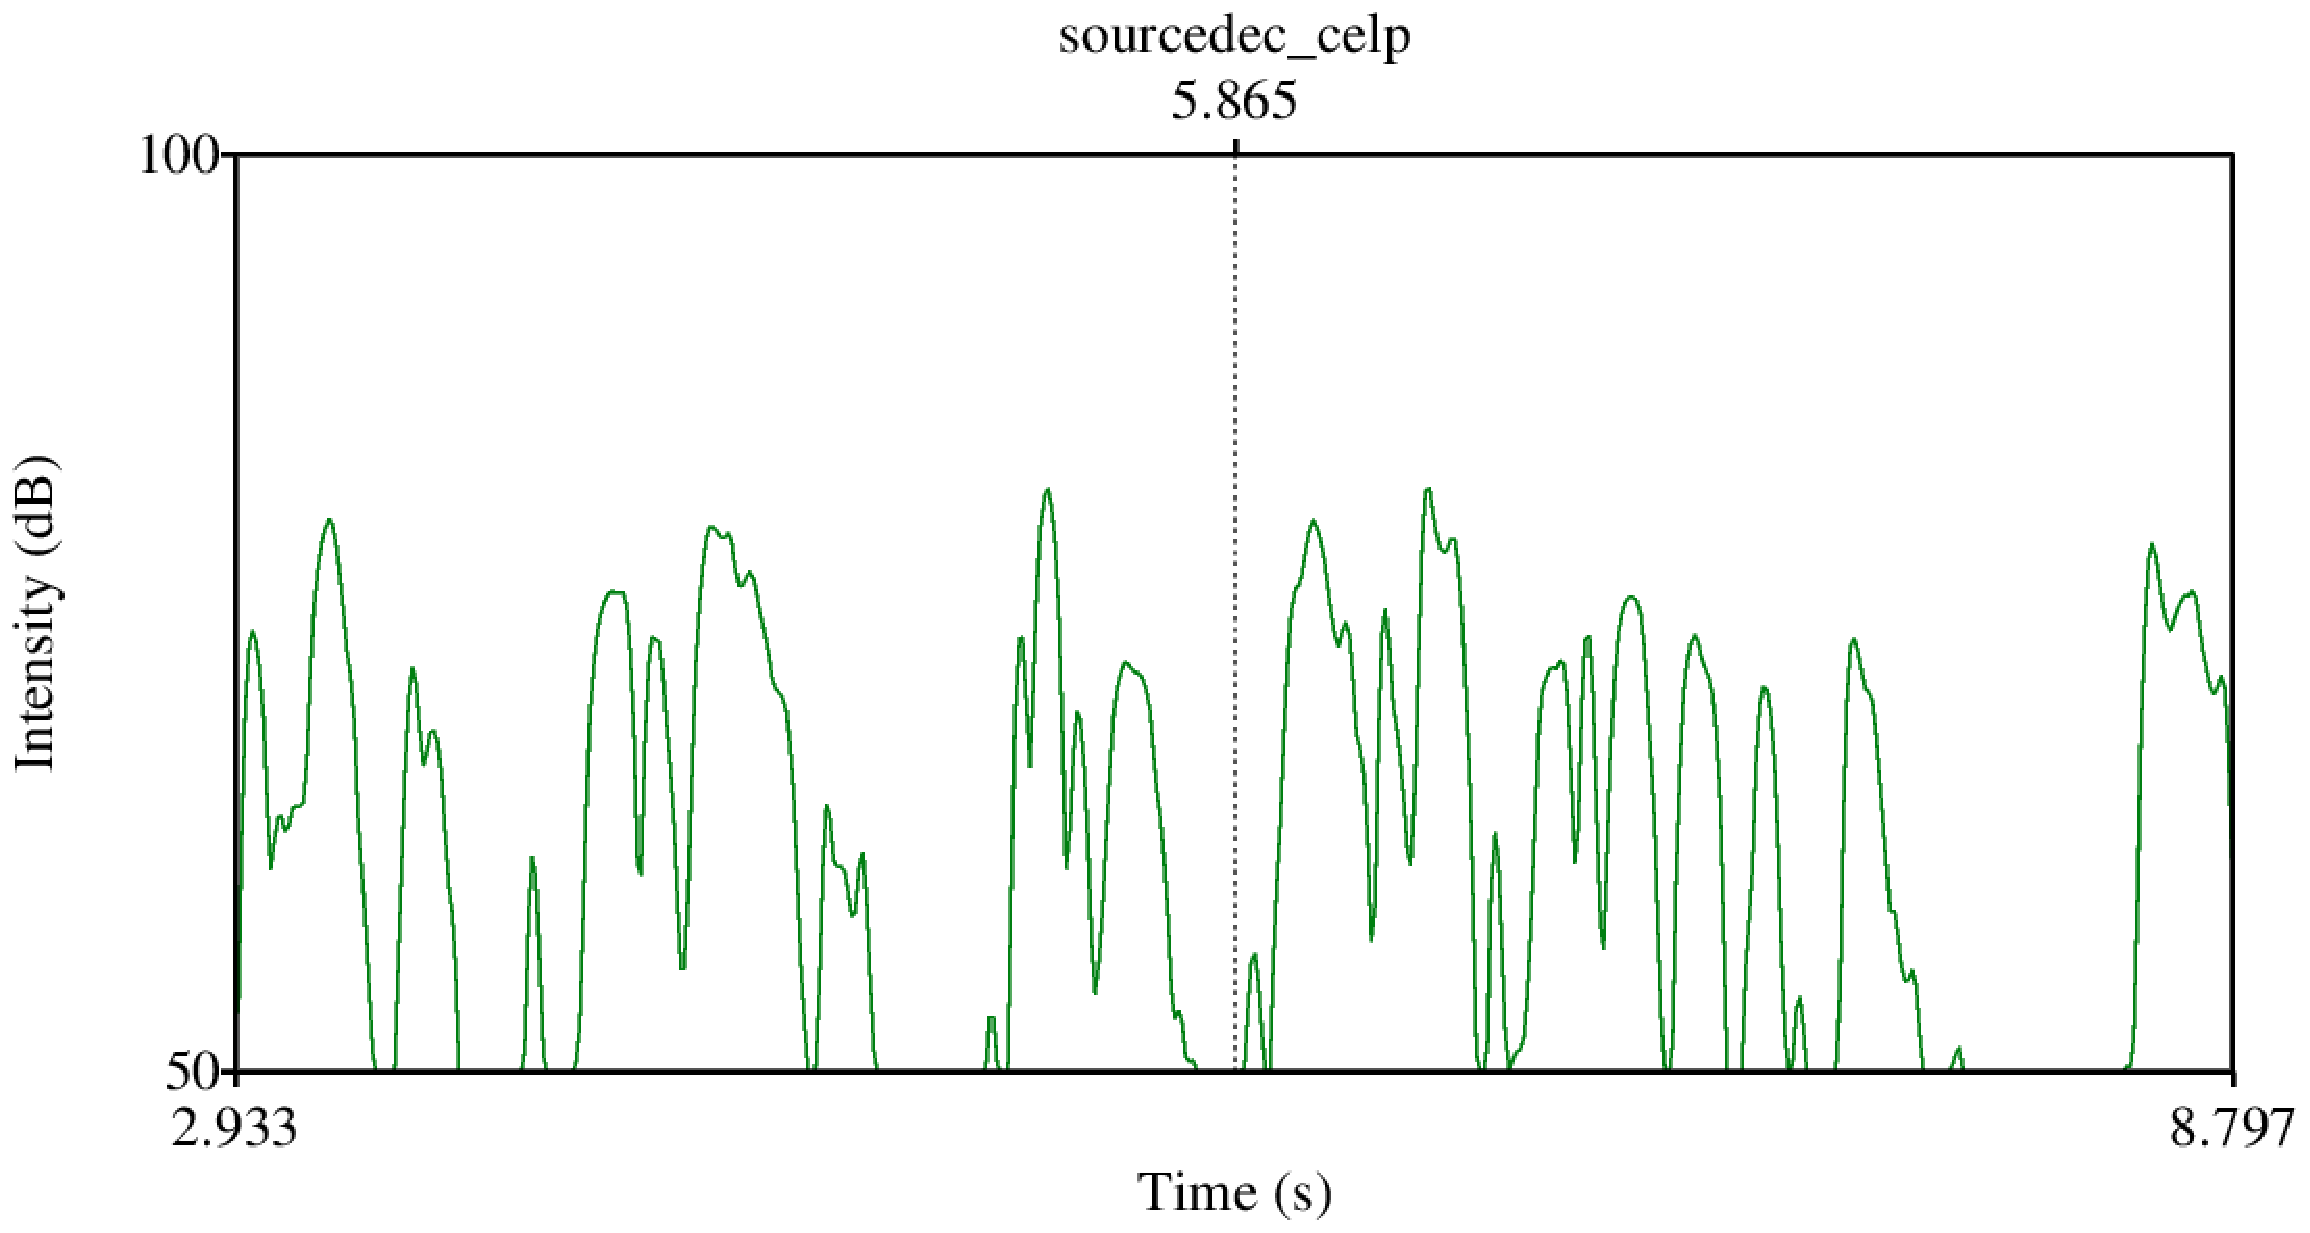
\includegraphics[width=4.5cm, height=3cm]{intcelp-eps-converted-to.pdf}%
%\label{fig:intcelp}
}}
\centerline{\subfigure[Decoder 2 output File]{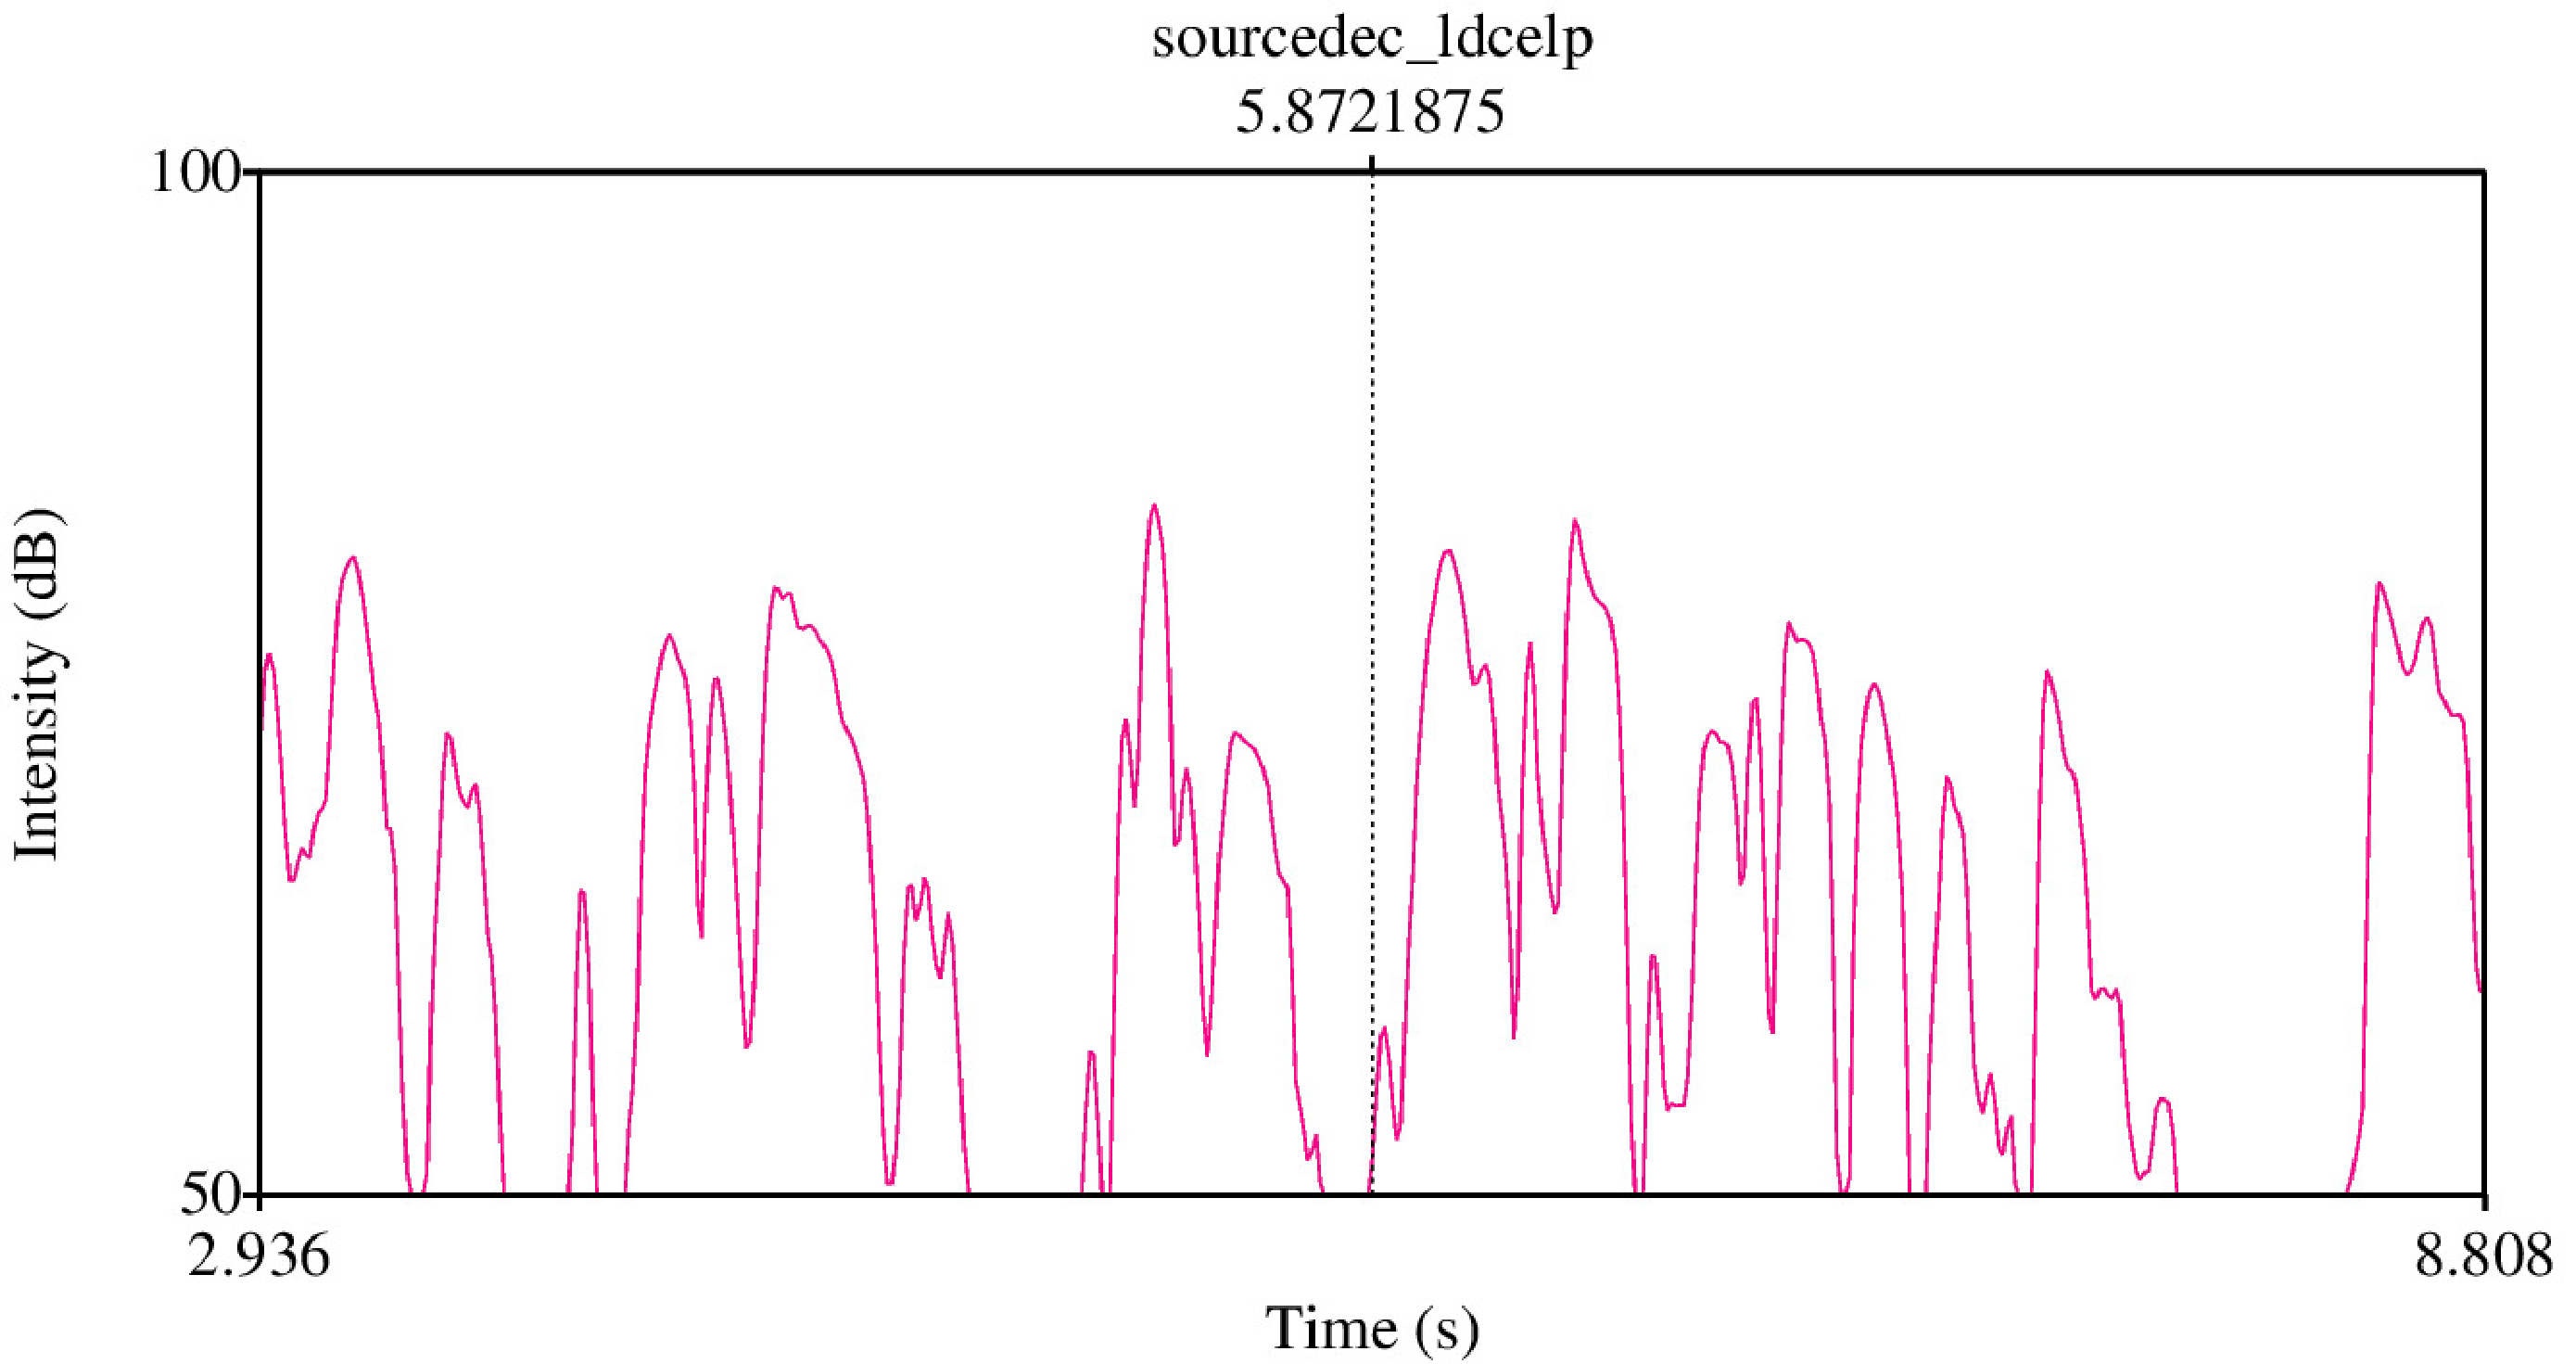
\includegraphics[width=4.5cm, height=3cm]{intldcelp-eps-converted-to.pdf}%
%\label{fig:intldcelp}
}
\hfil
\subfigure[Decoder 3 output file]{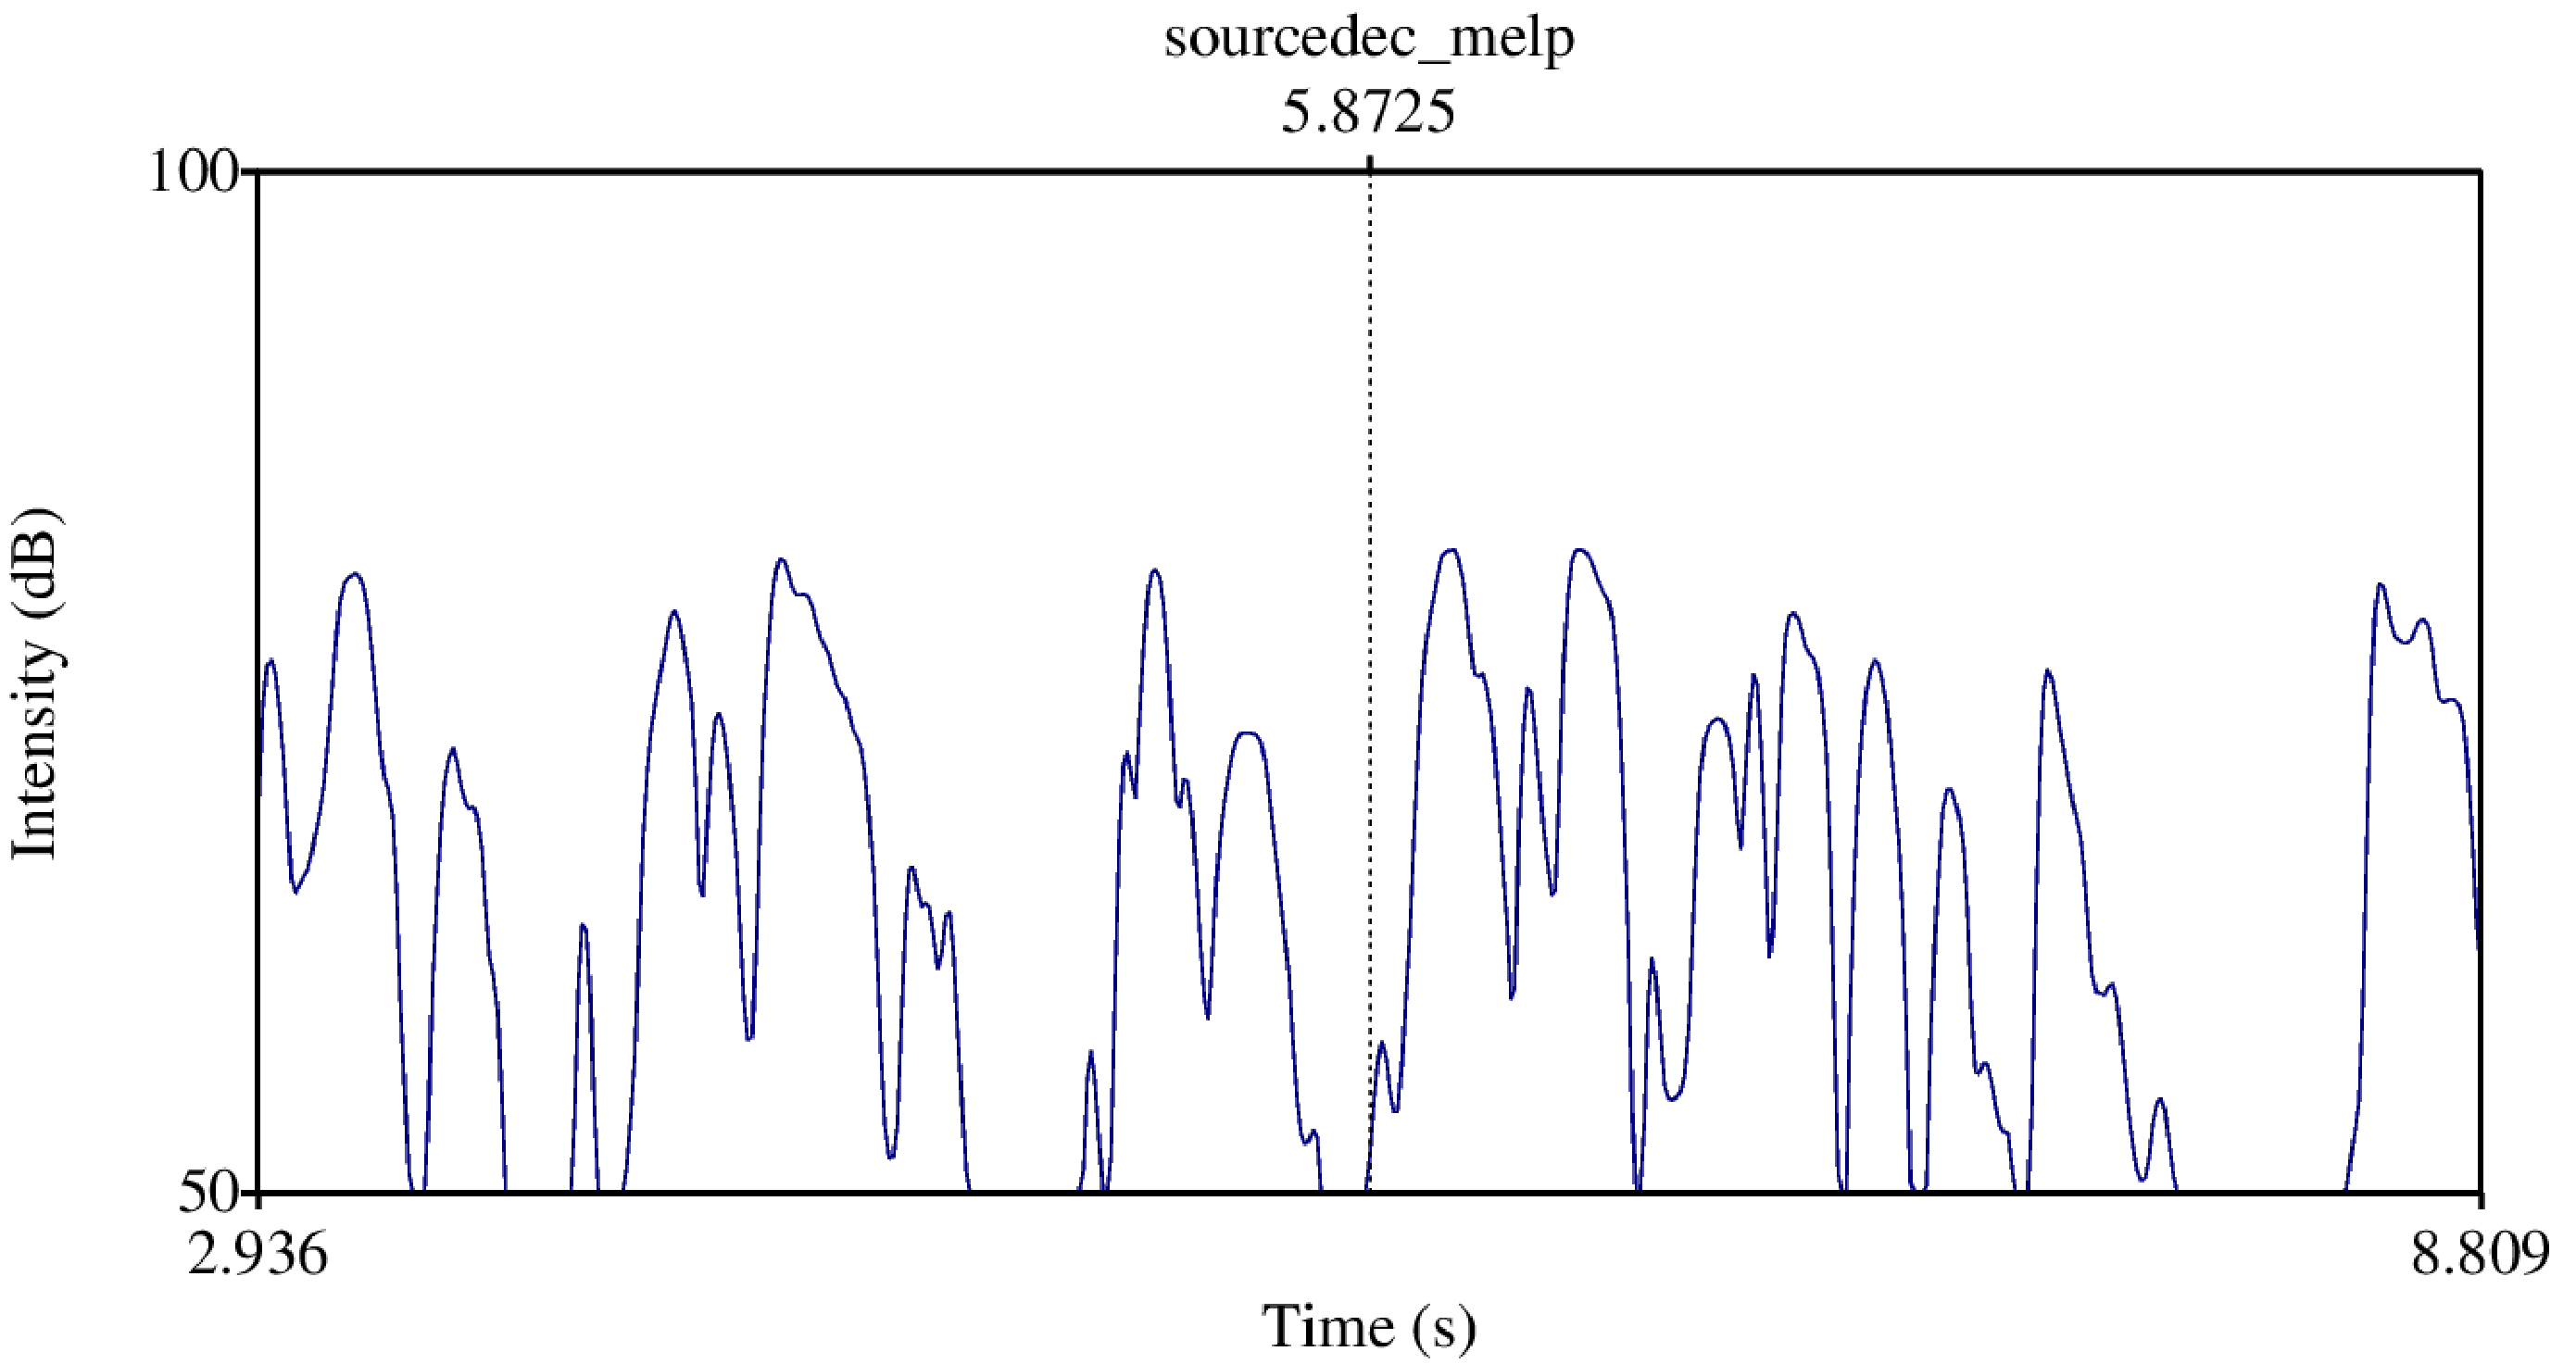
\includegraphics[width=4.5cm, height=3cm]{intmelp-eps-converted-to.pdf}%
%\label{fig:intmelp}
}
}
\caption{An Example showing Sub-figures}
\label{fig:int}
\end{figure*}


\subsubsection{Examples of tables}
\indent Tables may be formatted as in Table~\ref{tab:Table}.
\begin{table}[h]
	\renewcommand{\arraystretch}{1.1}
	\caption{An Example Table}
	\label{tab:Table}
	\centering
	\begin{tabular}{|c|c|c|c|}
		\hline
		Parameter 		& Algorithm 1 	&  	Algorithm 2 	& 	Algorithm 3	\\
		\hline

		file1.wav 		& 3.27		&	3.93		&	2.73 		\\
		file2.wav 		& 3.53		&	4.07		&	2		\\
		file3.wav 		& 3.53		&	4.47		&	2.8 		\\ \hline

		\hline 
		\textbf{Average Value}	& \textbf{3.44} &  \textbf{4.16} & \textbf{2.51}\\ \hline
	\end{tabular}
\end{table}


\indent If vertical lines are not required, tables may be formatted as in Table~\ref{tab:Table_novert}.
\begin{table}[h]
	\renewcommand{\arraystretch}{1.1}
	\caption{An Example Table}
	\label{tab:Table_novert}
	\centering
	\begin{tabular}{cccc}
		\hline
		Parameter 		& Algorithm 1 	&  	Algorithm 2 	& 	Algorithm 3	\\
		\hline

		file1.wav 		& 3.27		&	3.93		&	2.73 		\\
		file2.wav 		& 3.53		&	4.07		&	2		\\
		file3.wav 		& 3.53		&	4.47		&	2.8 		\\ \hline

		\hline 
		\textbf{Average Value}	& \textbf{3.44} &  \textbf{4.16} & \textbf{2.51}\\ \hline
	\end{tabular}
\end{table}



%-----include as many chapters as needed-----%

\chapter{Conclusion}\label{chapter:Conclusion}
\begin{flushleft}
	This report has attempted to provide a sufficient and elaborate introduction to DaxOS.\\
	The implementation has been discussed along with code samples where applicable.		
	The authors of this report hope that the explanations were clear and succinct.
	\vspace{1.5 cm}

	Interested readers can find the source code of this project at \url{https://github.com/DaxKernel/OS}.\\
	You can also check out our website at \url{https://daxkernel.github.io/}.
\end{flushleft}


\chapter{Appendix}\label{chapter:Appendix}
Include appendices here (optional)


\chapter{List of Publications}\label{chapter:List of Publications}
Write the list of publications here.

	\begin{enumerate}
    	\item Publication 1
	
    	\item Publication 2

    	\item Publication 3
  	\end{enumerate}

%%%-----BIBLIOGRAPHY-----%
%\addcontentsline{toc}{section}{REFERENCES}
%\bibliography{myreference}
%\bibliographystyle{IEEEtran}
%-----BIBLIOGRAPHY-----%
\include{REFERENCES}

\end{document}  % document ending 

%To run, go to the directory where the files are saved, and type:'latex FILENAME.tex' 
%To generate the PDF, type: 'dvipdfm FILENAME.dvi' 
%To generate the References page, type the following commands: 
%'latex FILENAME.tex' 
%'bibtex FILENAME.aux' 
%'latex FILENAME.tex' 
%'latex FILENAME.tex' 
%'dvipdfm FILENAME.dvi' 

